\documentclass{article}
%% PACKAGES %%

\usepackage{amsmath, amsfonts, amssymb, amsthm}
\usepackage{braket}
\usepackage{listings}
\usepackage{geometry}
\usepackage{xcolor}
\usepackage{textcomp}
\usepackage{graphicx}
\usepackage{fancyhdr}
\usepackage{sourcecodepro}
\usepackage{multirow}

%%%%%%%%%%%%%%

\hbadness = 99999 % remove annoying warning

\graphicspath{{./images}}

% Title Stuff
\title{ECE296 PLC Lab 1 - Traffic Stoplight}
\author{Chase A. Lotito, \textit{SIUC Undergraduate}}
\date{}

\begin{document}

\maketitle % Makes the title

\section{Introduction} 
% (Brief description of how the lab was setup and the steps you took while completing the tasks given)

This experiment was a nice use case of the programmable logic controller (PLC). Conventional stoplights are also controlled with PLCs, so it is fitting to implement a simple stoplight control system using the MicroLogix 1100B. 

For our stoplight system we have the following requirements: activate the current direction with I:0/0, keep the red light on for 30 seconds, the yellow light on for 5 seconds, the green light on for 15 seconds, and repeat this cycle to control the flow of traffic.

This design can be implemented using timers in the ladder logic. Timers have several logic bits associated with them: enable (EN), timing (TT), done (DN), and other values that we can utilize. We can start the red light timer via input switch I:0/0, and then control the other timers via their timer timing and timer done bits (e.g. T4:0.TT or T4:1.DN). By cascading timers like this, the traffic light logic is easily controllable and cyclic.

\section{Assessment of Design}
% (How did it work in the end? Any problems or missteps along the way? Explain key aspects of design. Attach images of working design.)

The specific ladder logic used can be seen in \textit{Appendix A}. 

Overall, the traffic light control system design works as expected, where after the light system's activation, the red light lights for 30 seconds, then the yellow light for 5 seconds, the green light for 15 seconds, and then repeating. Also, the red push-button was implemented as a RESET switch, and by pressing it, the cycle is restarted at the red light.

Figures \ref{fig:green}-\ref{fig:red}, show each light in use.

\begin{figure}[!ht] 
    \centering
    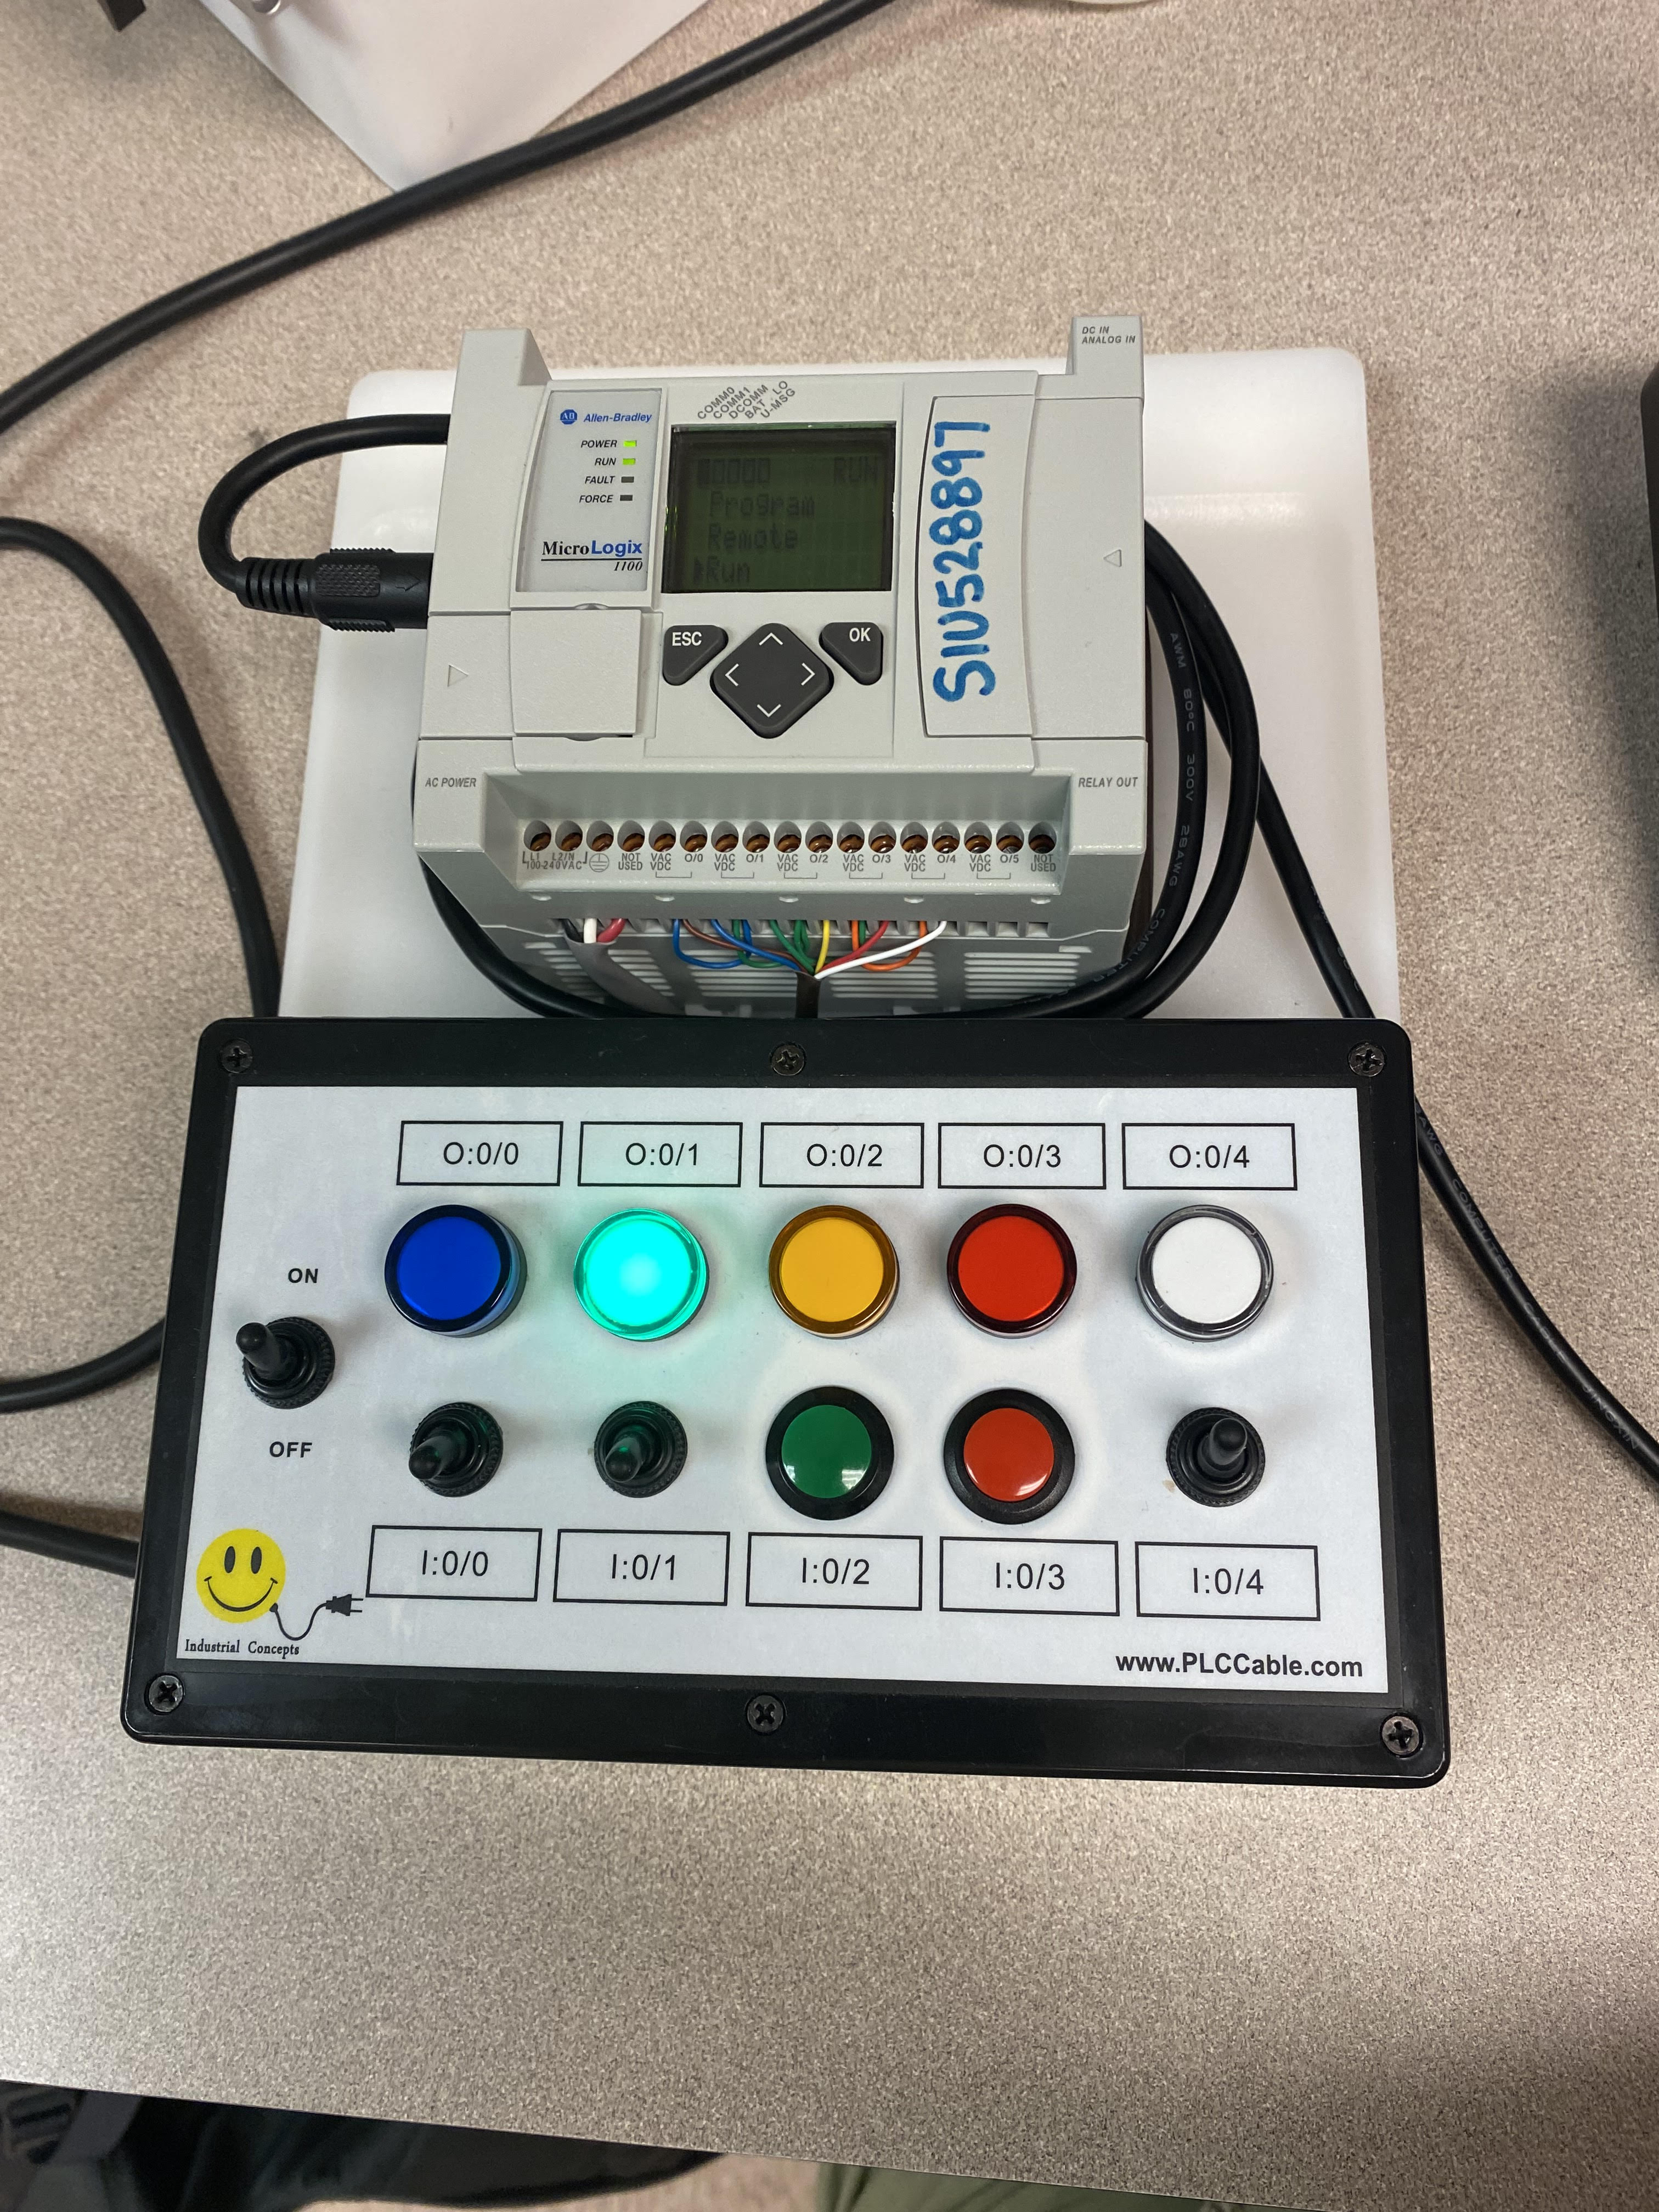
\includegraphics[width = 4cm]{green.jpg}
    \caption{Green light energized (GO).}
    \label{fig:green}
\end{figure}

\begin{figure}[!ht] 
    \centering
    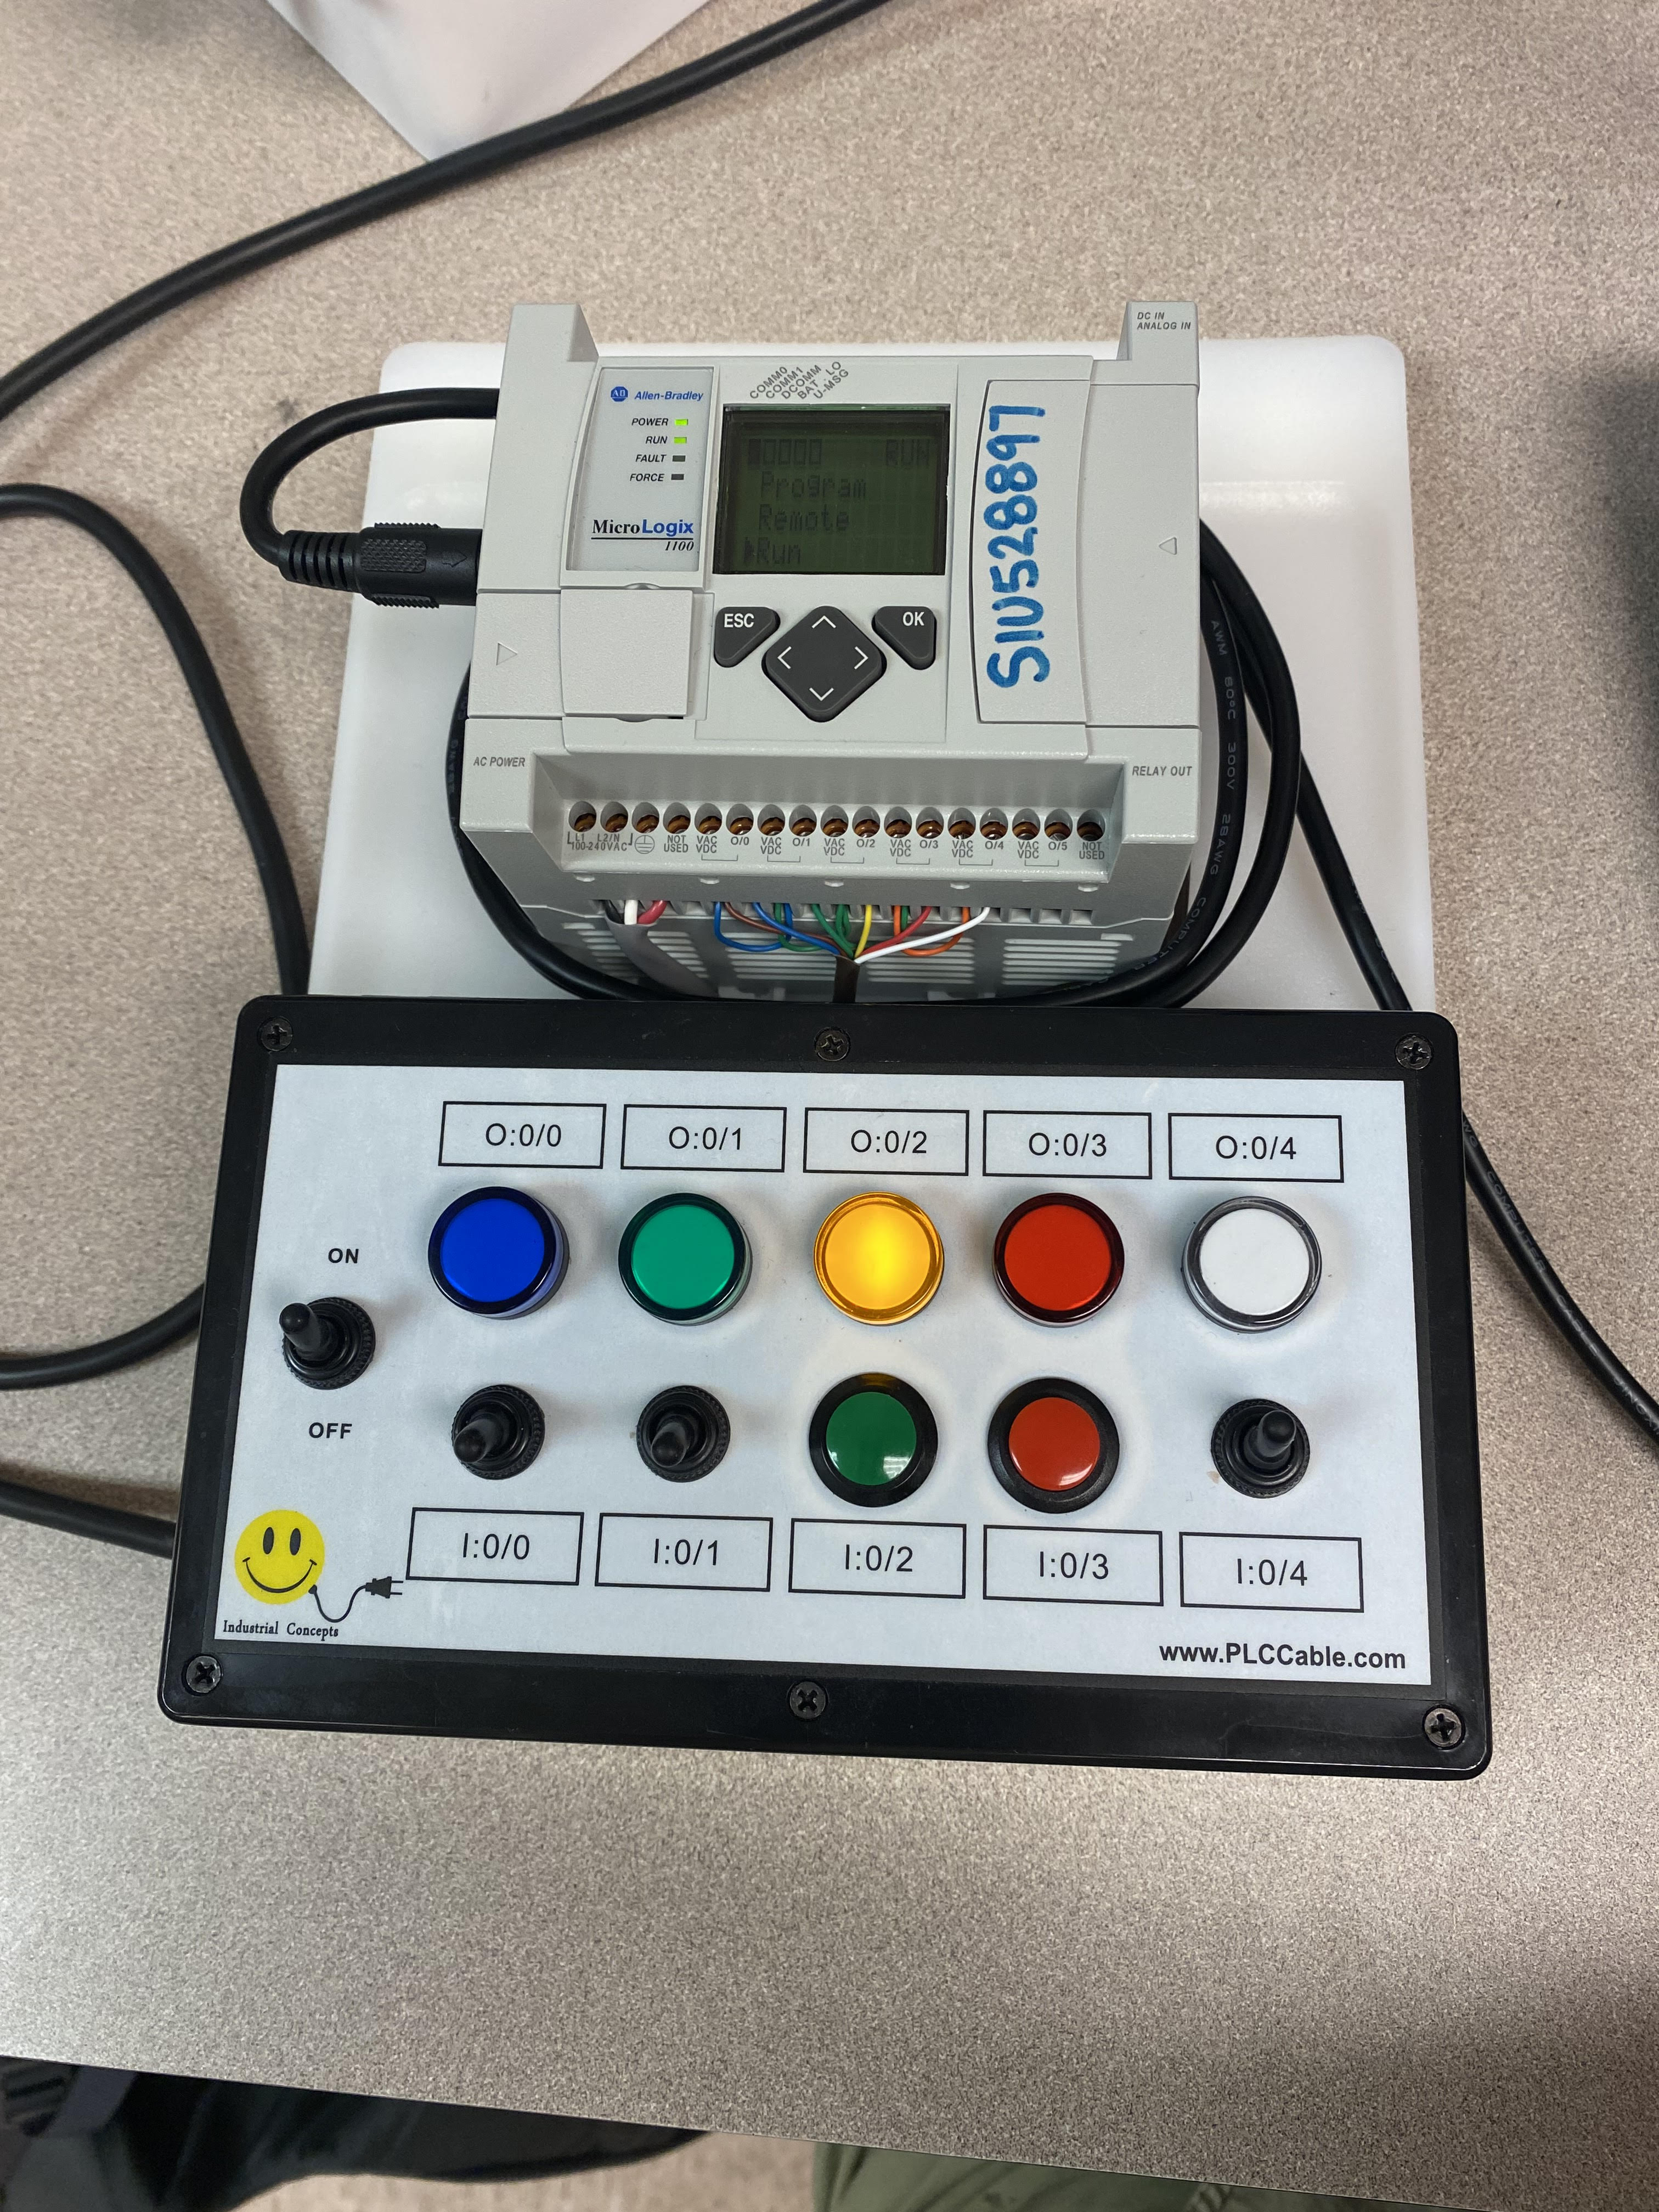
\includegraphics[width = 4cm]{yellow.jpg}
    \caption{Yellow light energized (SLOW).}
    \label{fig:yellow}
\end{figure}

\begin{figure}[!ht] 
    \centering
    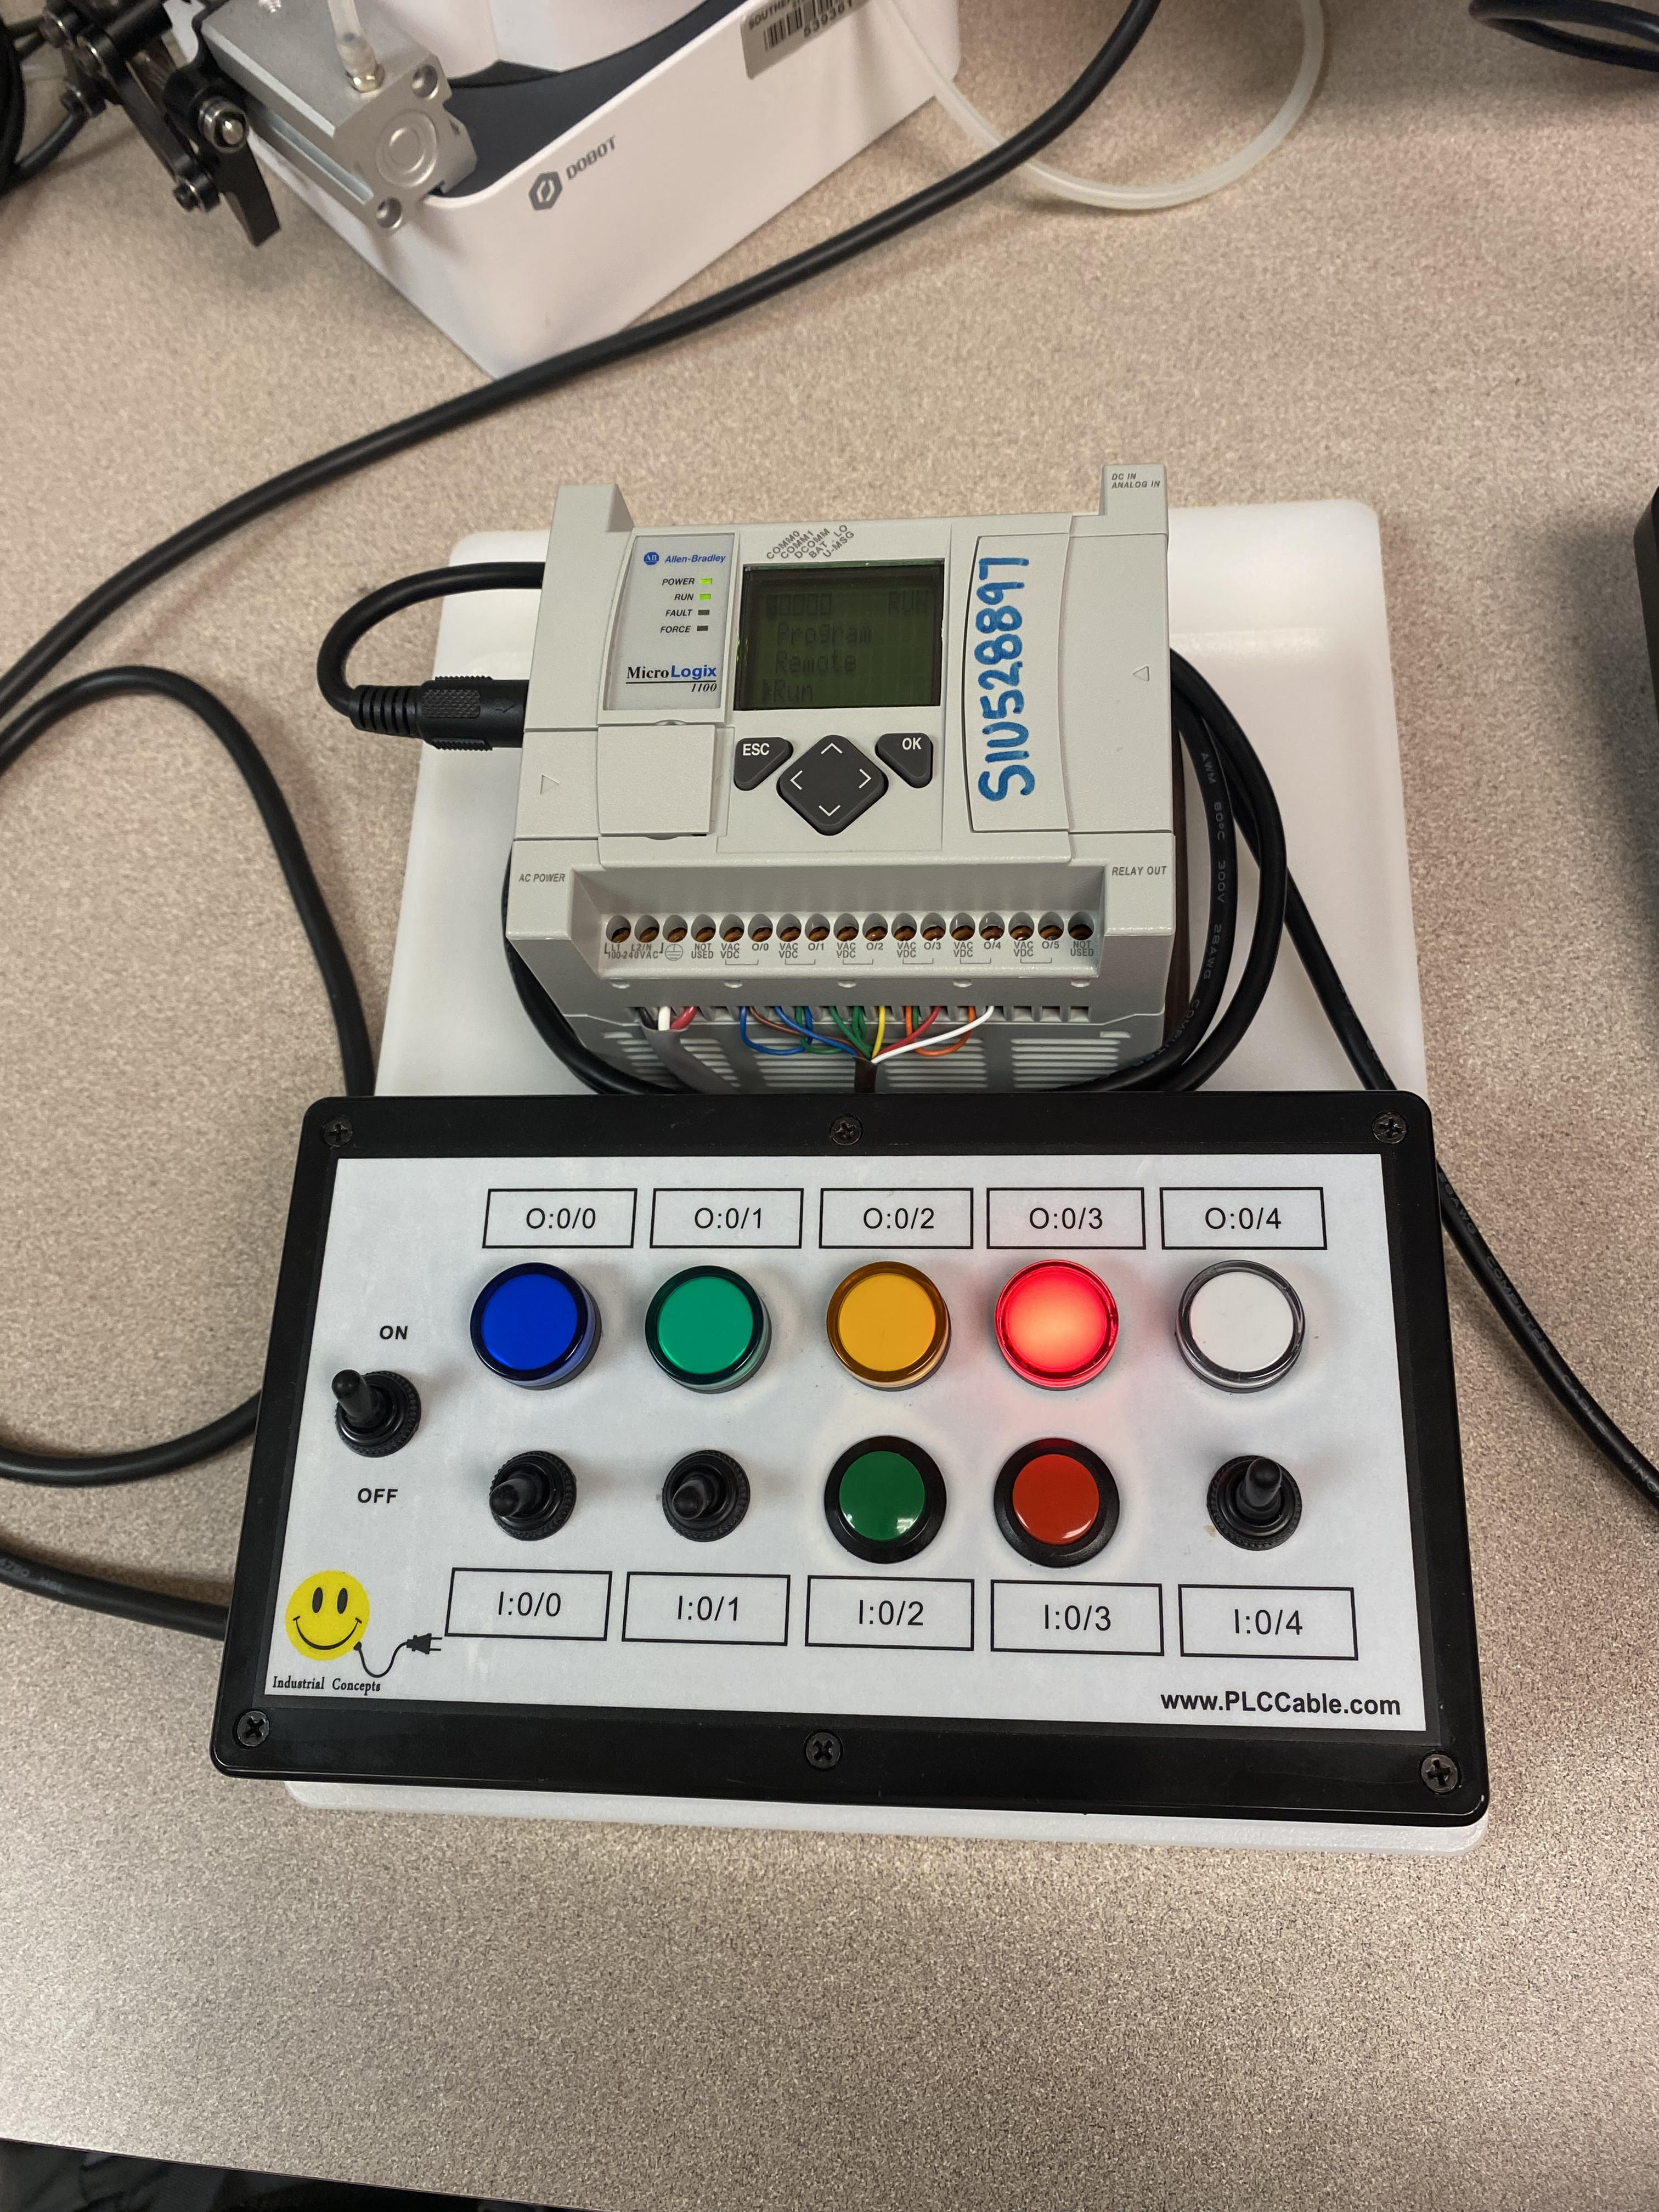
\includegraphics[width = 4cm]{red.jpg}
    \caption{Red light energized (STOP).}
    \label{fig:red}
\end{figure}

\section{Conclusion}
% (What did you learn during this lab? Final thoughts or findings? Did you meet the objectives? Answer any questions given in the lab manual here.)

This lab extended by knowledge of transient control of a system using programmable logic controllers. From this, any kinds of critical industrial systems can be implemented. Overall, this exercise gives an appreciation for the engineering that goes behind creating a robust control system, like traffic lights, which society depends on for safety and efficiency every single day.

I failed to implement a robust pedestrian walking system to coincide with the stoplight, which would be more accurate and add to the complexity of the design. However, using additional output latches would have made the timing for this possible.

\clearpage

\section*{Appendix A: Ladder Logic}

\begin{figure*}[h] 
    \centering
    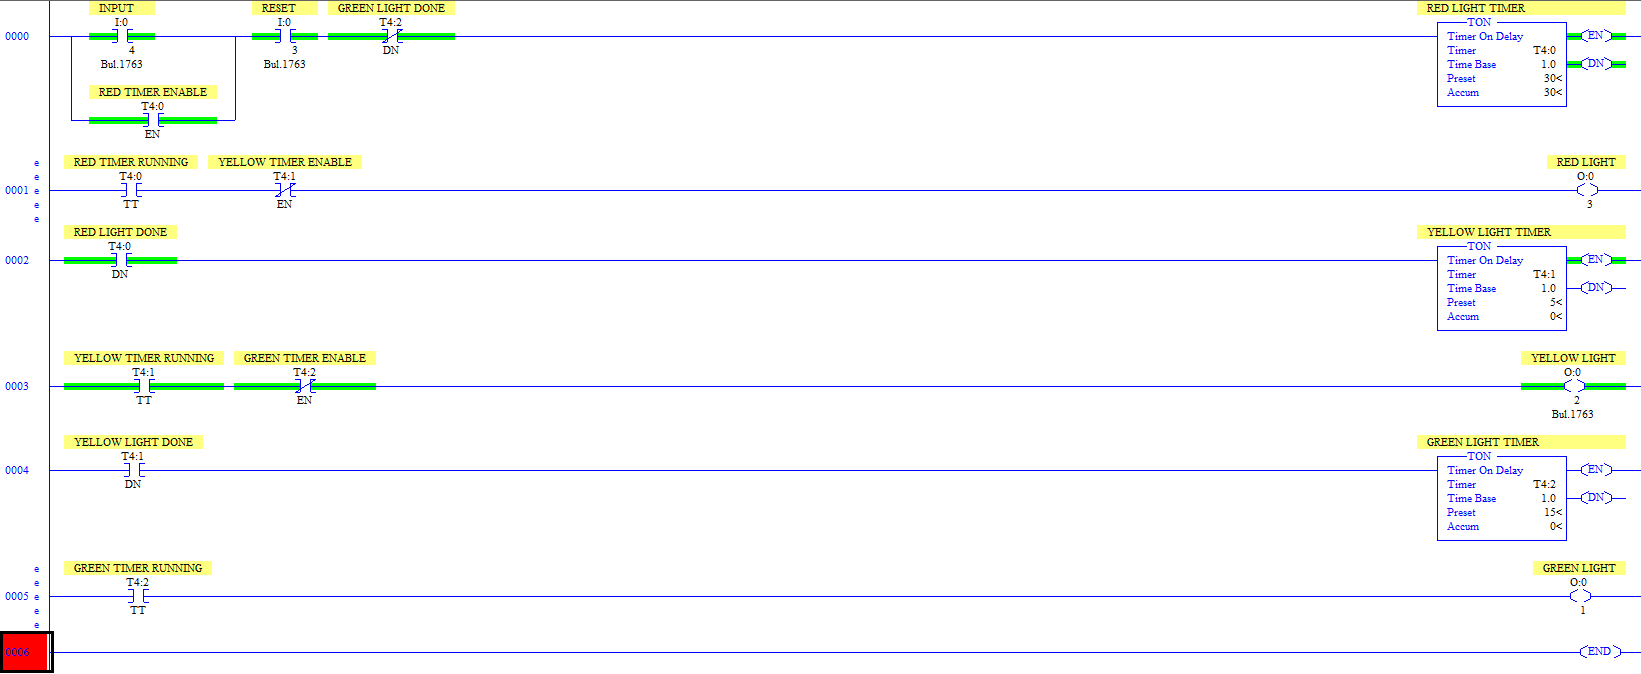
\includegraphics[width = 15cm]{ladderlogic.png}
    \caption{Ladder Logic for Stoplight}
    \label{fig:ladderlogic}
\end{figure*}

\end{document}
